\section{Bayesian augmentation results}\label{sec:augres}

Table~\ref{tab:augmentation} and Fig.~\ref{fig:aug} compare the four training conditions
on the identical set of held-out real papers.

Real-only training on the cohort gives MAE
$= 129.6 \pm 68.0$\,F\,g\textsuperscript{-1}. The
nominally best augmented condition (D, $+5.25\times$) reaches
123.6\,F\,g\textsuperscript{-1}, an improvement of
6.0\,F\,g\textsuperscript{-1}
(-4.6\%), improving MAE in
3 of 5 folds. The $+3\times$ condition
is the \emph{worst} of the four.

\subsection{Why this improvement is not robust}
Three observations, all visible in Fig.~\ref{fig:noise}, place the apparent gain inside the
configuration noise.

\begin{enumerate}
\item \textbf{Re-drawing the synthetic set moves the score by more than the effect.}
Holding fold, ratio and network degree fixed and changing only the generator seed shifts
fold MAE by 12.3\,F\,g\textsuperscript{-1} on average --- larger than the
6.0\,F\,g\textsuperscript{-1} attributed to the best ratio.
\item \textbf{Changing the network degree moves it as much as changing the ratio.} At fixed
ratio, varying $k \in \{1,2,3\}$ changes MAE by up to
17.8\,F\,g\textsuperscript{-1}, while the entire spread across the four
augmentation ratios is 15.1\,F\,g\textsuperscript{-1}. Two nuisance
parameters and the treatment produce effects of the same magnitude.
\item \textbf{The response is not monotone in the amount of synthetic data.} The ordering
is $+5.25\times$, real-only, $+1\times$, $+3\times$. A genuine regularisation benefit would
not place the middle ratio last.
\end{enumerate}

Paired Wilcoxon signed-rank tests across the five folds were computed
(\texttt{06\_statistical\_comparison.csv}), but with five paired folds the smallest
attainable two-sided $p$-value is $2^{-4} = 0.0625$, so no comparison here can reach
$p<0.05$ by construction. The $p$-values are reported for completeness only; the effect
direction, its consistency across folds and its size relative to the noise floor are the
meaningful quantities, and none supports the augmentation.

\paragraph{Conclusion.} Bayesian-network augmentation did not produce robust evidence of
improved prediction on unseen real papers at any ratio tested. This is reported as found: no
configuration search was run to make the synthetic data appear beneficial, and the largest
augmentation ratio was not preferentially reported.

\begin{figure*}[htbp]\centering
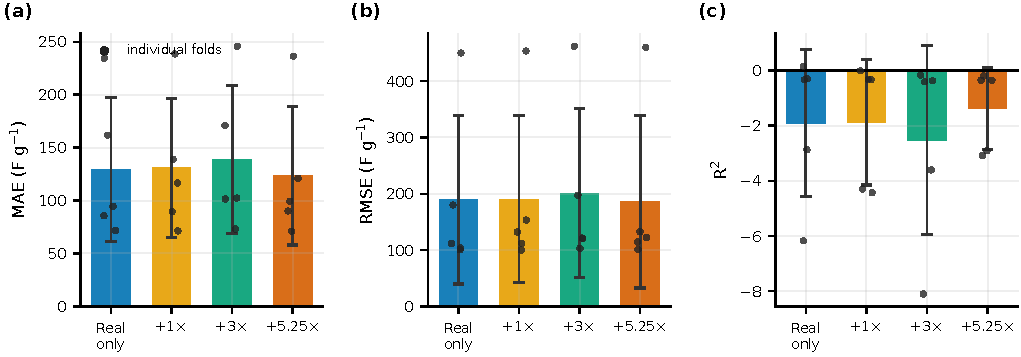
\includegraphics[width=\textwidth]{figures/fig03_augmentation_comparison.pdf}
\caption{Real-only versus augmented training on unseen real papers ($k=2$; bars are means
over five grouped folds, error bars the fold-to-fold SD, points the individual folds).
(a) MAE, (b) RMSE, (c) $R^2$. The conditions are indistinguishable relative to the
fold-to-fold spread.}
\label{fig:aug}\end{figure*}

\begin{figure*}[htbp]\centering
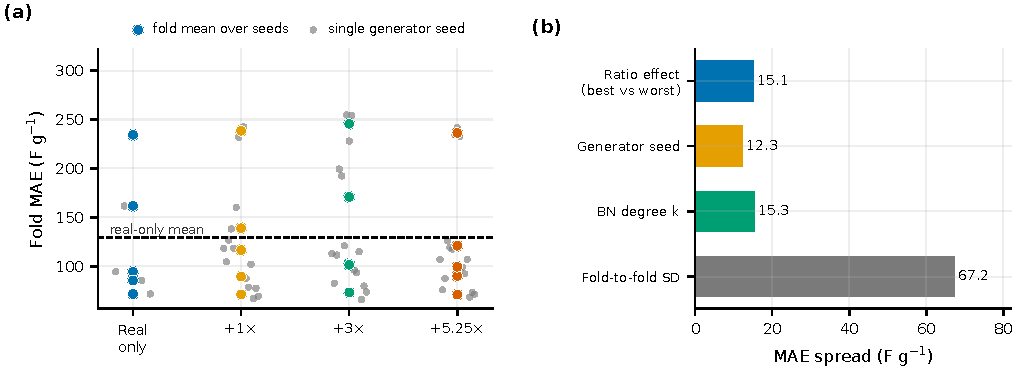
\includegraphics[width=\textwidth]{figures/fig05_generator_uncertainty.pdf}
\caption{The apparent augmentation effect against the noise it must be judged against.
(a) Fold MAE for every generator seed (grey) and the fold mean over seeds (coloured); the
dashed line is real-only training. (b) The best-versus-worst ratio effect compared with the
spread produced by re-drawing the synthetic set, by changing the Bayesian-network degree, and
by fold-to-fold variation. The treatment effect is indistinguishable in magnitude from the two
nuisance sources and is an order of magnitude below the fold-to-fold spread.}
\label{fig:noise}\end{figure*}

\begin{table}[htbp]
\centering
\caption{Real-only versus Bayesian-augmented training, evaluated on the identical set of held-out real papers in every condition ($k=2$, five grouped folds, three independent generator seeds averaged per fold). Errors in F\,g\textsuperscript{-1}; $\pm$ denotes the fold-to-fold SD.}
\label{tab:augmentation}
\footnotesize
\begin{tabular}{lrrrrrr}
\toprule
\textbf{Training set} & \textbf{$n_{\mathrm{syn}}$} & \textbf{$R^2$} & \textbf{MAE} & \textbf{RMSE} & \textbf{Pooled MAE} & \textbf{Seed SD} \\
\midrule
Real only & 0 & -1.91 $\pm$ 2.67 & 129.6 $\pm$ 68.0 & 189.1 $\pm$ 149.3 & 129.5 & -- \\
Real $+\,1\times$ & 38 & -1.88 $\pm$ 2.27 & 130.9 $\pm$ 65.4 & 190.2 $\pm$ 148.6 & 130.8 & 11.1 \\
Real $+\,3\times$ & 113 & -2.53 $\pm$ 3.43 & 138.7 $\pm$ 69.8 & 200.8 $\pm$ 150.3 & 138.6 & 18.9 \\
Real $+\,5.25\times$ & 198 & -1.38 $\pm$ 1.48 & 123.6 $\pm$ 65.5 & 186.1 $\pm$ 153.5 & 122.8 & 6.9 \\
\bottomrule
\end{tabular}
\par\vspace{2pt}\begin{minipage}{\linewidth}\scriptsize ``Seed SD'' is the within-fold MAE standard deviation across the three generator seeds, i.e.\ the score movement produced by re-drawing the synthetic set alone. It is of the same magnitude as the entire spread between augmentation ratios, and for the $+3\times$ condition it exceeds it.\end{minipage}
\end{table}
